\documentclass{article}
\usepackage[a4paper]{geometry}
\usepackage[spanish]{babel}
\usepackage{parskip}
\usepackage{setspace}
\usepackage{graphicx}
\usepackage{fancyhdr}
\geometry{total={6in, 9in}}
\usepackage{makeidx}
\usepackage{lscape}
\usepackage{pdflscape}
\usepackage{fancyhdr}
\usepackage{pdfpages}
\usepackage{rotating}
\usepackage{etoolbox}
\usepackage{listings}
\usepackage{float}
\usepackage{caption}
\usepackage{subcaption}

\lstdefinestyle{customc}{
  language=C++,
  showstringspaces=false,
  basicstyle=\footnotesize\ttfamily,
  keywordstyle=\bfseries\color{green!40!black},
  commentstyle=\itshape\color{purple!40!black},
  identifierstyle=\color{blue},
  stringstyle=\color{orange},
}

\lstset{escapechar=@,style=customc}

\newcommand{\tabitem}{%
  	\usebeamertemplate{itemize item}\hspace*{\labelsep}}
\usepackage[hidelinks]{hyperref}

%HEADRULE

\pagestyle{fancy}
\setlength{\headheight}{30.2pt}
\setlength{\headsep}{30pt}
% INICIO DE PÁGINAS
\begin{document}
\begin{titlepage}
	
	
	\begin{center}
		{\LARGE \textbf{UNIVERSIDAD NACIONAL DE INGENIERÍA}}\\
		\vspace{5 mm}
		{\large \textbf{Facultad de Ingeniería Industrial y de Sistemas}}\\
		\vspace{15.5 mm}
		\begin{figure}[h]
			\centering 
			
\includegraphics[width=0.45\textwidth]{images/CiberSecFIIS.png}
		\end{figure}
		\vspace{4 mm}	
		{\Large \textbf{Informes de exploración de vulnerabilidades en HTB} }\\
		\vspace{5 mm}
		
		\onehalfspacing  % Espaciamiento 1.5
		{\Large \textbf{``{\@De las máquinas: OpenAdmin, Fuse \\Magic, Remote }''} }\\
		
		\singlespacing  % Fin del espaciamiento 1.5
		
		\vspace{4 mm}	

		\vspace{20 mm}
		{\large \textbf{ELABORADO POR:} }\\
		\vspace{10 mm}
		\begin{center}
			\begin{minipage}{0.7\textwidth}
			  \begin{itemize}
				\item \Large Alfonso Suárez, Luis
				\item \Large Mottoccanche Tantaruna, Joseph
				\item \Large Chi Jon, Lau
			  \end{itemize}
			\end{minipage}
		  \end{center}

		\vspace{5 mm}	
	\end{center}

\end{titlepage}


\clearpage
\tableofcontents
\clearpage
% ----------------------------Time-----------------------------------
\section{Friendzone}
\subsection{Enumeración}
Lo primero a realizar en cualquier máquina es un escaneo rápido con nmap, para esto usamos el comando con los parámetros:
\begin{itemize}
	\item -p-
	\item --min-rate=5000
	\item -v
	\item -oN puertos.txt
	\item -sV 
	\item -sC 
\end{itemize}
\begin{figure}[H]
	\center
	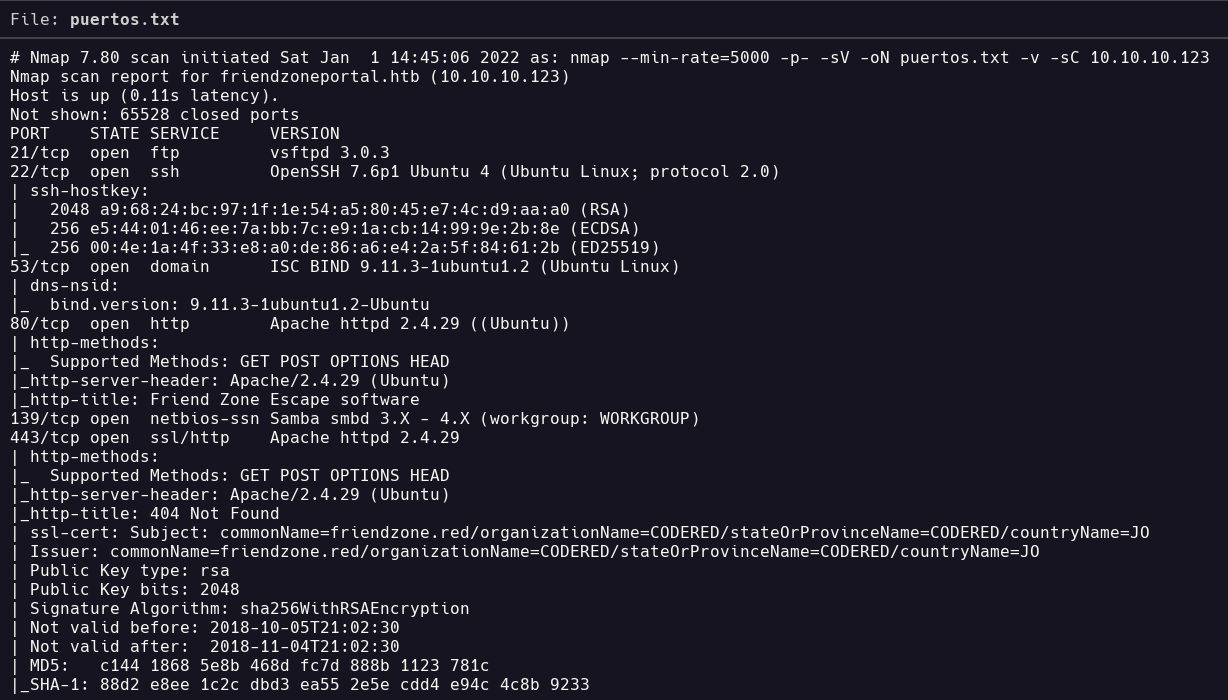
\includegraphics[width=\textwidth]{images/friendzone/puertos-nmap.png}
	\caption{escaneo con nmap}
\end{figure}
Encontramos el puerto 80 y el 443 abiertos, pero este último aparece con un nombre de dominio específico, así que vamos a darle un vistazo.
\begin{figure}[H]
	\center
	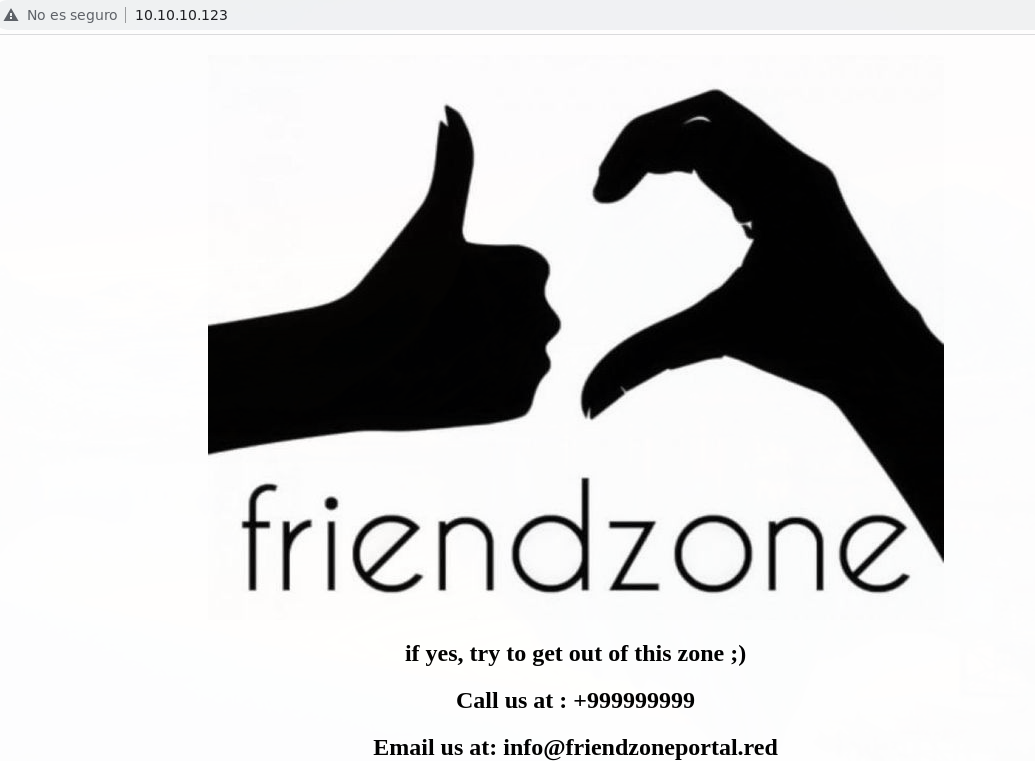
\includegraphics[width=\textwidth]{images/friendzone/puerto80.png}
	\caption{página del puerto 80}
\end{figure}
Para poder mostrar la página del 443 necesitamos primero modificar el /etc/hosts y añadirle el dominio que sale en el escaneo que es "friendzone.red".
Pero al hacer eso vemos que tiene otra página, entonces ya sabemos que es un vhost y para hallar el resto usaremos la técnica de transferencia de zona, "afxr".

\begin{figure}[H]
	\center
	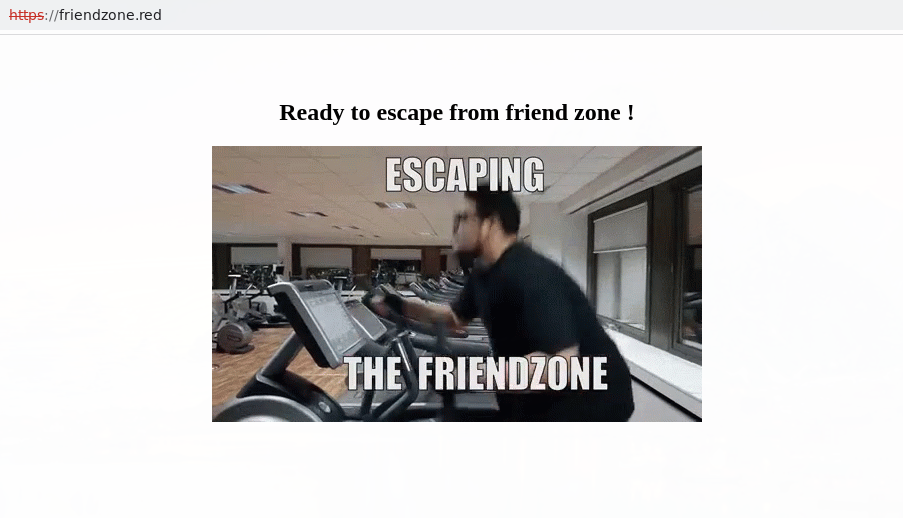
\includegraphics[width=\textwidth]{images/friendzone/puerto443.png}
	\caption{página del puerto 443}
\end{figure}

Necesitamos entonces usar el comando dig que es una utilidad que viene al instalar "dnsutils" junto con nslookup, luego de instalarlo y ejecutarlo con el parámetro axfr, nos muestra lo siguiente.

\begin{figure}[H]
	\center
	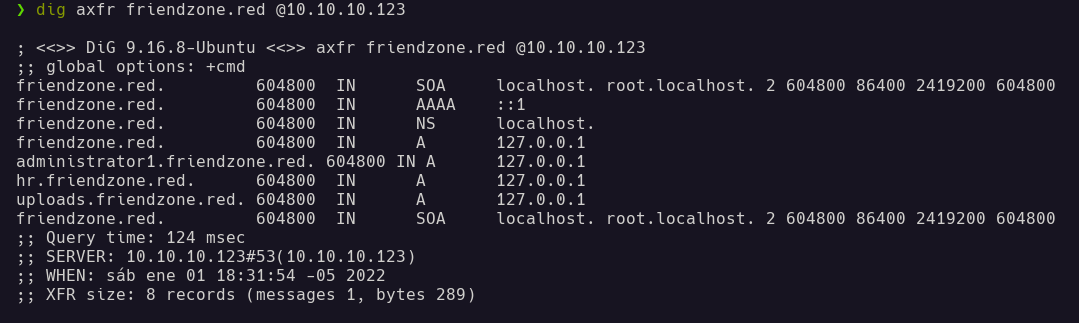
\includegraphics[width=\textwidth]{images/friendzone/dig-information.png}
	\caption{resultado ejecución dig}
\end{figure}



\begin{figure}[H]
	\center
	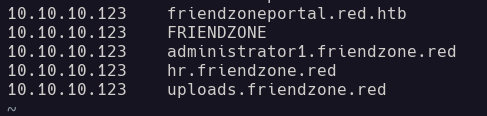
\includegraphics[width=\textwidth]{images/friendzone/modificacion-hosts.png}
	\caption{modificación /etc/hosts}
\end{figure}

Entonces dentro de estos vemos las páginas que están disponibles y encontramos las siguientes: 

\begin{itemize}
	\item hr.friendzone.red
	\item upload.friendzone.red
	\item administrator1.friendzone.red
\end{itemize}

Vimos que entrando a administrator1.friendzone.red encontramos un login, pero nos faltan las credenciales y no hemos tenido mucha información para obtenerla.
por lo que tocó investigar un poco los otros puertos, y descubrimos el puerto samba en el 445.

\begin{figure}[H]
	\center
	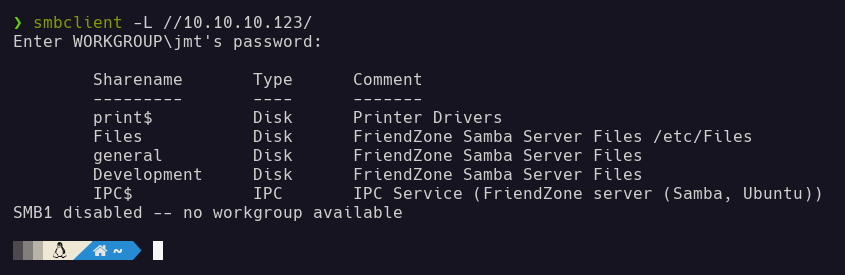
\includegraphics[width=\textwidth]{images/friendzone/samba-escaneo.png}
	\caption{listado de directorios en samba}
\end{figure}

Tenemos algunos directorios enumerados, pero solo tenemos permiso de lectura y escritura en dos, en "general" y "Development", algo que nos llama la atención es que "Files" es referenciado como "/etc/Files", los cual podría indicar una subida directa al /etc.


\begin{figure}[H]
	\center
	\includegraphics[width=\textwidth]{images/friendzone/conexión-general-samba.png}
	\caption{acceso a "general"}
\end{figure}

Pero más interesante lo que encontramos dentro, fue un "creds.txt" lo cual suena muy prometedor sin embargo, no lo podemos ver directamente.

\begin{figure}[H]
	\center
	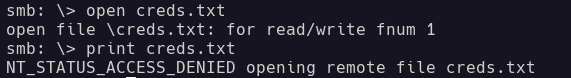
\includegraphics[width=\textwidth]{images/friendzone/intento-lectura-samba.png}
	\caption{intento de lectura}
\end{figure}

Entonces lo descargamos con el comando "get" del smbclient, y una vez descargado ya lo podremos leer.
Una vez descargado vimos que contiene credenciales de lo que parece un usuario administrador.

\begin{figure}[H]
	\center
	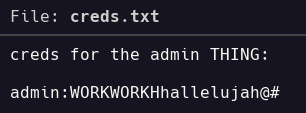
\includegraphics[width=\textwidth]{images/friendzone/cat-creds.png}
	\caption{lectura creds.txt}
\end{figure}

Probamos entonces con el ftp a ver si tenemos suerte, pero no obtuvimos nada.

\begin{figure}[H]
	\center
	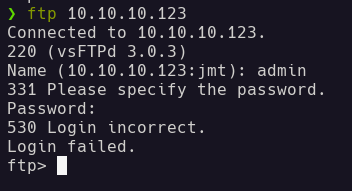
\includegraphics[width=\textwidth]{images/friendzone/login-ftp-fallido.png}
	\caption{fallo login ftp}
\end{figure}

Pero nos dimos cuenta que realmente las credenciales eran de la página de login en "administrator1.friendzone.red"

\begin{figure}[H]
	\center
	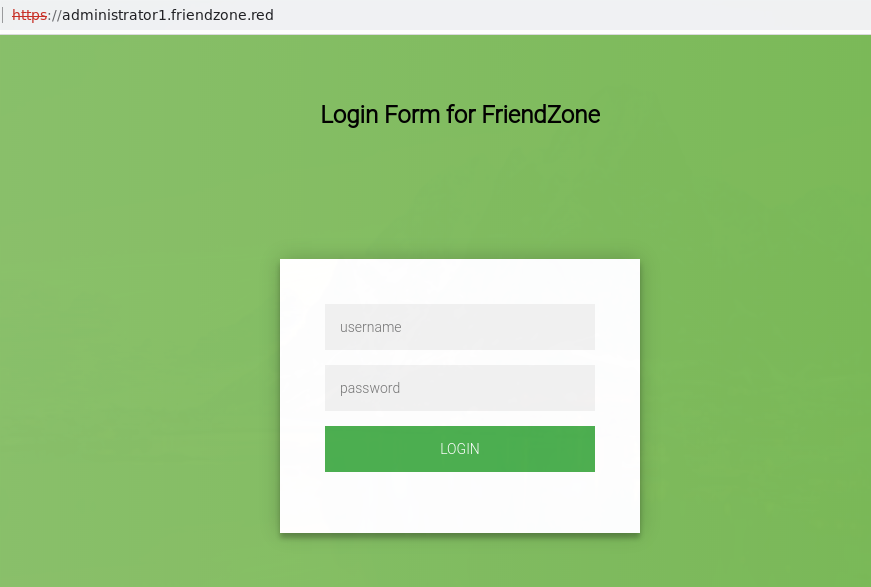
\includegraphics[width=\textwidth]{images/friendzone/login-administrator.png}
	\caption{fallo login ftp}
\end{figure}

Una vez logueados vemos que nos dice que nos redirigamos a "dashboard.php"

\begin{figure}[H]
	\center
	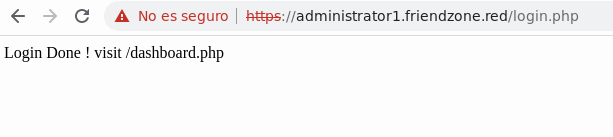
\includegraphics[width=\textwidth]{images/friendzone/login-correcto.png}
	\caption{fallo login ftp}
\end{figure}

\subsection{Explotación}

Dentro del dashboard nos dan instrucciones de cómo deberíamos redirigirnos a la imagen apuntando a un timestamp para controlar, vemos que este timestamp es una página eh php que ejecuta el servidor cada vez que apuntas a él, esto lo sabemos gracias a un escaneo de directorios a la ruta "administrator1.friendzone.red"

Entonces podemos subir una página php que ejecute una reverse shell y apuntar a esta en lugar del timestamp, pero para subir esta página hay dos formas:
\begin{itemize}
	\item usando el "upload.friendzone.red".
	\item subiendo por samba a un directorio que permita escritura.
\end{itemize}

Tuve un problema con el upload.friendzone.red ya que había realizado demasiadas consultas, así que intenté con la otra forma.

\begin{figure}[H]
	\center
	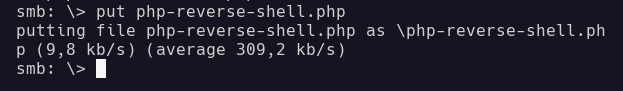
\includegraphics[width=\textwidth]{images/friendzone/subiendo-reverse.png}
	\caption{subiendo mediante samba la reverse shell}
\end{figure}

Esta reverse shell la pueden encontrar del siguiente github: "https://github.com/d4t4s3c/Offensive-Reverse-Shell-Cheat-Sheet".

Entonces solo quedaría correr un nmap en escucha con el comando "nmap -lvnp 1234".
y luego ejecutar la ejecución en la página.

\begin{figure}[H]
	\center
	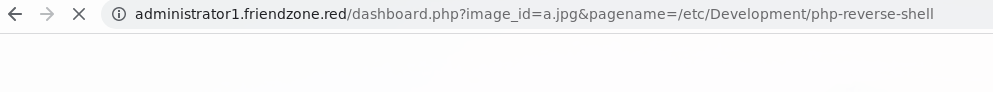
\includegraphics[width=\textwidth]{images/friendzone/ejecucion-reverse.png}
	\caption{ejecutando la reverse shell}
\end{figure}

y obtenemos la conexión luego de esto.

\begin{figure}[H]
	\center
	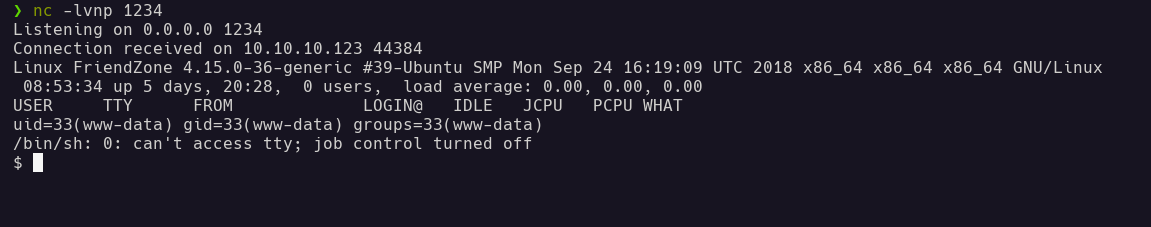
\includegraphics[width=\textwidth]{images/friendzone/shell-obtenida.png}
	\caption{obtención de shell}
\end{figure}

Ya con esto es suficiente para leer el "user.txt" del usuario friendzone, lo cual es un poco raro porque solo somos www-data cuando entramos al dispositivo.

\begin{figure}[H]
	\center
	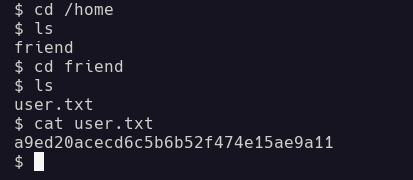
\includegraphics[width=\textwidth]{images/friendzone/flag-user.png}
	\caption{flag del user friendzone}
\end{figure}


\subsection{Escalamiento de privilegios}




\end{document}
